\chapter{Support Vectors Machine}

\section{Algorithm background}

SVM belong to the class of maximum margin classifiers. They perform pattern recognition between two classes by finding a decision surface that has maximum distance to the closest points in the training set which are termed support vectors.

We start with a training set of points $x_{i} \in R$, $i = 1,2 ... N$ where each point $x_{i}$ belongs to one of two classes identified by the label $y \in { {1,-1} }$ Assuming that data is linearly separable, the goal of SVM is to separate the two classes by a hyperplane.

\begin{figure}[H]
\centering
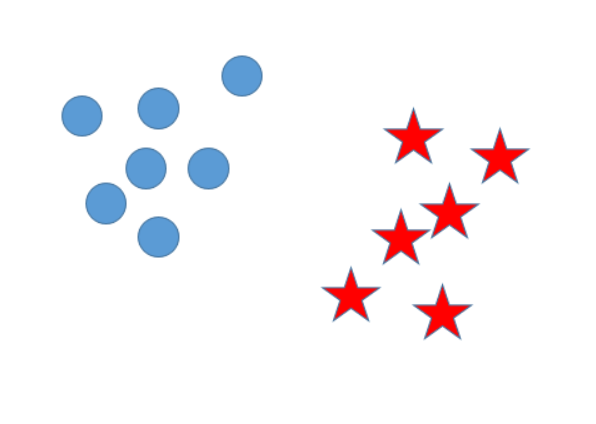
\includegraphics[scale=0.5]{img/svm/linear.png}
\caption{Linearly separable dataset and its hyperplane}
\end{figure} 

The hyperplane is a set of points satisfying equation 4.1

\begin{equation}
f(x) = w^T x + b = 0
\end{equation}

The vector $w$ is known as the weight vector, and $b$ is called the bias. 
Suppose the weight vector can be expressed as a linear combination of the training examples, i.e.

\begin{equation}
w = \sum_{i=1}^{N} \alpha_{i}x_{i}
\end{equation}

Then:

\begin{equation}
f(x) = \sum_{i=1}^{N} \alpha_{i}x_{i}^T x + b
\end{equation}

The representation in terms of the variables $\alpha_{i}$ is known as the dual representation of the decision boundary.

The hyperplane divides the space into two: the sign of the discriminant function  denotes the side of the
hyperplane a point is on.

\subsection{The geometric margin}
For a given hyperlane we denote by $x_{+}$ the closest point to the hyperpalne among the positive examples and by $x_{-}$ the closest point to the hyperpalne among the negative examples. These points are commonly called support vectors.
The margin of a hyperplane f can be described as:

\begin{equation}
m(f) = \frac{1}{2}\uvec{w}^{T}(x_{+}-x_{-}) 
\end{equation}

where $\uvec{w}$ is a unit vector in the direction of w. We assume that $x_{+}$ and $x_{-}$ are equidistant from
the hyperplane:

\begin{equation}
f(x_{+}) = w^Tx_{+} + b = a
f(x_{-}) = w^Tx_{-} + b = -a
\end{equation}

where $a>0$

Adding the two equations and dividing by $||w||$ we can describe the geometric margin as:
\begin{equation}
m(f) = \frac{1}{||w||}
\end{equation}

The purpose of the algorithm is to maximize the geometric margin. This optimization problem can be also seen as minimizing $||w||^2$

\begin{equation}
\begin{multlined}
\min_{w,b} \frac{1}{2}||w||^2 \\
s.t. \forall i, y_{i}(w^Tx_{i} + b) \geq 1
\end{multlined}
\end{equation}

The constraints in this formulation ensure that the maximum margin classifier classifies each example correctly. However, in our optimization problem we want to introduce some kind of "penalty" for data misclassification. This can be done with changing our optimization problem to so-called soft-margin SVM:

\begin{equation}
\begin{multlined}
\min_{w,b} \frac{1}{2}||w||^2 + C \sum_{i=1}^{N} \xi_{i}\\
s.t. \forall i, y_{i}(w^Tx_{i} + b) \geq 1 - \xi_{i}
\end{multlined}
\end{equation}

where $\xi_{i}\geq 0$ are so-called \textit{slack variables} that allow an example to be in the margin ($0\leq \xi_{i}\geq 1$, also called a margin error) or to be misclassified ($\xi_{i} > 1$).

\begin{figure}[H]
\centering
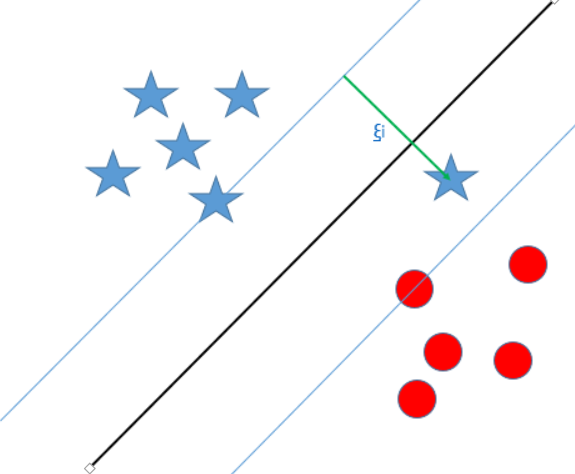
\includegraphics[scale=0.5]{img/svm/ksi.png}
\caption{Illustration of $\xi$ value}
\end{figure} 

The parameter C is called \textit{slack penalty} and is one of the SVM "tuning" parameters.

The solution to this optimization problem can be solved using Lagrange duality principle.

Classification of a new data point is performed by computing the  (?) equation with previously optimized parameters.

\begin{equation}
h_{w,b}(x) = g(w^T x + b)
\end{equation}

where $w$ and $b$ are coefficients of the hyperplane trained by SVM algorithm and $g(z)=1$ if $z\geq0$, and $g(z)=-1$ otherwise.


\subsection{Non linear separable dataset}

The described approach works only for linearly separable data set. Nevertheless, in many applications a non-linear classifier is required. Linear classifiers have several advantages, one of them being that they often have simple training algorithms. 
This begs the question: Can we extend the entire linear-classifier construction to generate non-linear decision boundaries? 

\begin{figure}[H]
\centering
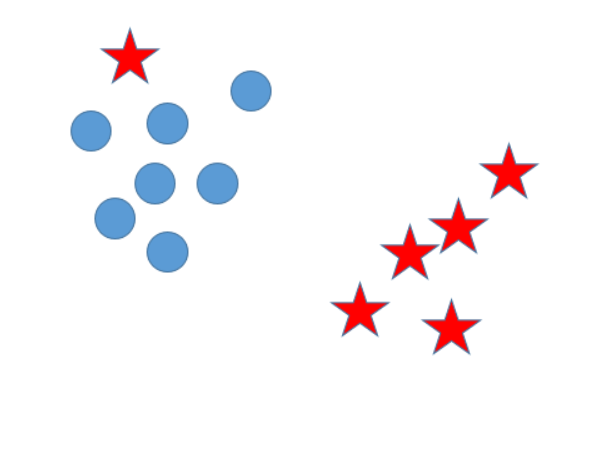
\includegraphics[scale=0.5]{img/svm/nonlinear.png}
\caption{Nonlinearly separable dataset and its hyperplane}
\end{figure} 

The solution to this problem is to map our data from
the input space X to a feature space F using a non-linear function $\phi : X \rightarrow F$, so that the entire construction can be extended to the case of nonlinear separating surfaces. 

Each point $x_{i}$ in the input data is mapped to a point $z = \phi(x)$ of a higher dimensional space, called the feature space.

Rather than applying SVMs using the original input attributes x, we learn the algorithm using new features $\phi(x)$ instead.

To map our training set into the higher dimensional space we choose the similarity 

For each $x_{i}$ we calculate the similarity value between this  and every other sample in the data set. The similarity function is also called a kernel.

\begin{equation}
\begin{multlined}
\\
f_{i1} = K(x_{i}, x_{1})\\
f_{i2} = K(x_{i}, x_{2})\\
\vdots\\
f_{iN} = K(x_{i}, x_{N})
\end{multlined}
\end{equation}

In the new high dimensional space each point $x_{i}$ is represented as a vector:

\begin{equation}
\vec{f_{i}} = [f_{i1}, f_{i2}, \cdots, f_{iN}]
\end{equation}

In the feature space, F expression 4.3 takes the form:

\begin{equation}
f(x) = \sum_{i=1}^{N} \alpha_{i}\phi(x_{i})^T \phi(x) + b
\end{equation}
The feature space F may be very high dimensional, hence computing the whole equation becomes computationally expensive unless the kernel function K, defined by equation( ??) can be computed efficiently.
\begin{equation}
K(x,z) = \phi(x)^T\phi(z)
\end{equation}

Using the kernel function the decision boundary function can be defined as: 

\begin{equation}
f(x) = \sum_{i=1}^{N} \alpha_{i}K(x, x_{i})+ b
\end{equation}

Two most widely used kernels are:
\begin{enumerate}
\itemsep0em 
\item Gaussian kernel
\begin{equation}
K(x,x_{i}) = exp(-\frac{||x-x_{i}||^2}{2\sigma^2})
\end{equation}
where $\sigma$ is a parameter that controls the width of Gaussian
\item Polynomial kernel 
\begin{equation}
K(x,x_{i}) = [(x \cdot x_{i} + 1]^d
\end{equation}
with degree d
\end{enumerate} 


\subsection{Multi-class classification problem}

There are two basic approaches for solving n-class problems with SVMs:
\begin{enumerate}
\itemsep0em 
\item one-vs-all approach - q SVMs are trained. Each of the SVMs separates a single class from all remaining classes.
\item pairwise approach - q(q-1)/2 SVMs are trained. Each SVM separates a pair of classes. The pairwise classifiers are arranged in trees, where each tree node represents an SVM. 
\end{enumerate}

\subsection{Face recognition}
The system has a linear SVM for every person in the database. Each SVM is trained to distinguish between all images of a single person and all other images. Given a set of q people and a set of q SVMs, each one associated to one person, it is relatively easy to perform recognition. Specifying the threshold, the distance between input and given SVM models are computed as follows:

\begin{equation}
d(x) = \frac{•\sum_{i=1}^l \alpha_{i}y_{i}x_{i} \cdot x + b}{||\sum_{i=1}^l\alpha_{i}y_{i}x_{i}||}
\end{equation}

We can notice that numerator is equal to right side of equation (12), hence the sign of $d$ is the classification result for x, and $||d||$ is the distance from x to the hyperplane.

The class label of input picture is computed as follows:

$y = \begin{cases} n$ if $d_{n}(x) > t \\$ not recognized if $d_{n}(x) \leq t \end{cases}$

where $d_n(x) = max ({d_{i}}_{i=1}^q)$

\section{Implementation and test results}

The SVM algorithm was implemented with Python 3.6.1 with usage of numpy, PIL and sklearn libraries. 

The first step in the algorithm is data preprocession. As in the Multilayered Perception approach, the images were preprocessed with PCA algorithm in order to reduce the dimensionality of input data, hence reducing the computational complexity of the algorithm. The algorithm is using one-vs-one approach.

The tests were performed on two different databases: 
\begin{itemize}
\itemsep0em 
\item Chicago Face Database - pictures captured in controlled environment
\item Labeled Faces in Wild database - pictures captured in uncontrolled environment, with various lightning conditions, pose, facial expression etc. 
\end{itemize}

The main goal of the experiments was to examine the influence of parameter $C$ and different kernels on accuracy of the algorithm.

\section{Tests on pictures captured in controlled environment}

The database was divided into training and testing samples. The training was performed using 3 pictures of the individual, one picture was used to test the trained model. 

\subsection{20 individuals}

The first experiment was performed on 20 individuals from CFD database. 
The Gaussian and Polynomial kernels were tested. 

The Gaussian kernel as a similarity function that measures the “distance” between a pair of examples, ($x_{i}$, $x_{j}$). The Gaussian kernel is also parameterized by a bandwidth parameter $\sigma$ (equation(???), which determines how fast the similarity metric decreases to 0 as the examples are further apart. 

The kernel function from equtaion (???) can be also interpreted as:

\begin{equation}
exp(-\gamma * ||x-x_{i}||^2)
\end{equation}

where:
\begin{equation}
\gamma = \frac{1}{2\sigma^2}
\end{equation}

The influence of $\gamma$ parameter on the gaussian kernel function can be visualized as presented on figure (??). (with the smallest value of $\gamma$ on the most left graph and the greatest on the right) 


\begin{figure}[H]
\centering
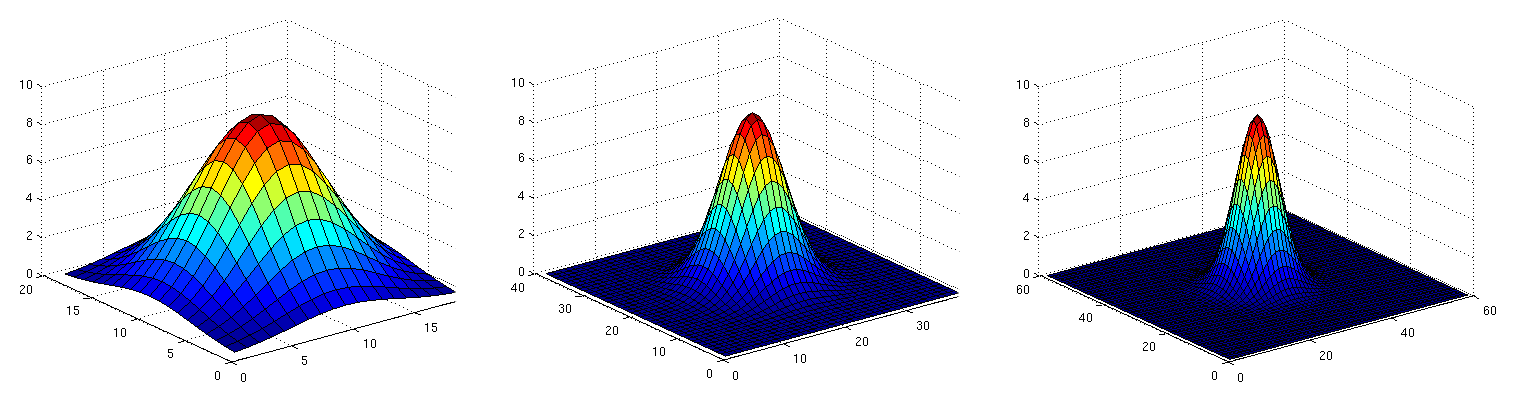
\includegraphics[scale=0.27]{img/svm/gaussian.png}
\caption{Gaussian kernel visualization}
\end{figure} 

The figure(??) presents the SVM training accuracy with varying $\gamma$ and C parameter:

\begin{figure}[H]
\centering
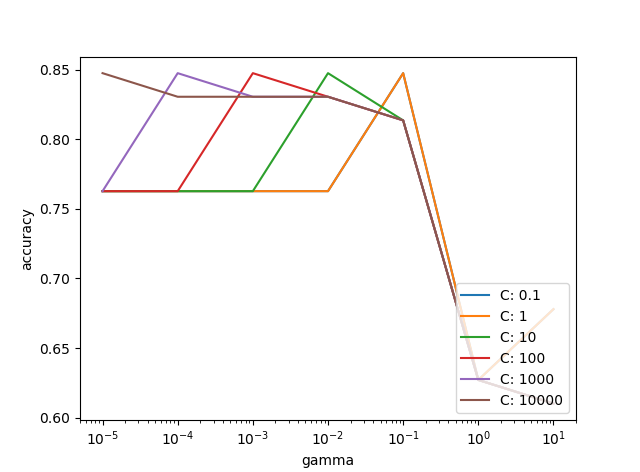
\includegraphics[scale=0.75]{img/svm/better_graphs/CFD_20i_rbf.png}
\caption{Training score with varying gamma and C parameter for 20 individuals}
\end{figure} 


The best score (~0.85) was obtained with several configurations of $C$ and $\gamma$ parameters. The further testing was performed with $C = 10^3$ and $\gamma = 10^-4$

In this configuration SVM algorithm reached 80\% of recognition rate on the testing samples.

The same experiment was performed with usage of polynomial kernel. 
The influence of polynomial degree was examined and is presented on figure (??).

\begin{figure}[H]
\centering
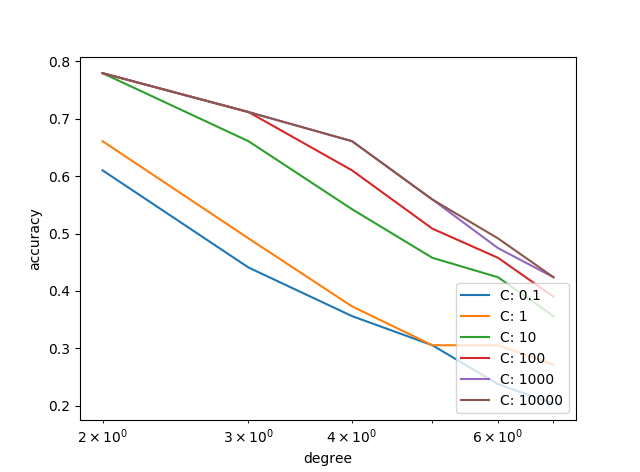
\includegraphics[scale=0.75]{img/svm/better_graphs/CFD_20i_poly.png}
\caption{Training score with varying polynomial degree and C parameter for 20 individuals}
\end{figure} 

On Figure(7.6 (??)) we can see that our data can be nicely separated with polynomial of second degree.  
The recognition rate was tested on SVM trained with $C = 10$ and the degree = 2.

Obtained result is ~70\%, which is 10 percentage points less than result of SVM trained with Gaussian kernel. 

\subsection{40 individuals}

The same test scenario was used to examine SVM on bigger amount of input data - 40 individuals.

The results are presented below.

\begin{figure}[H]
\centering
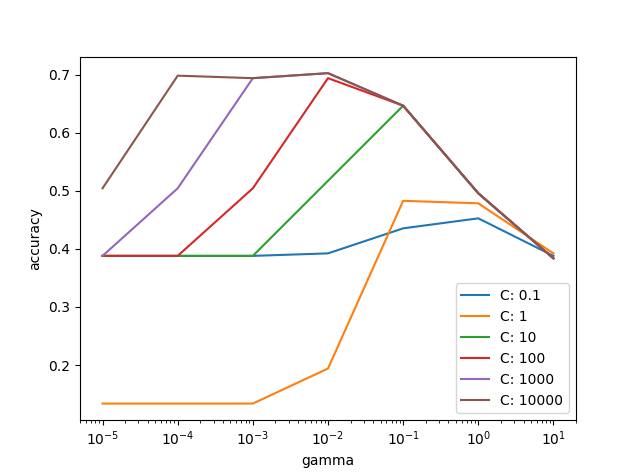
\includegraphics[scale=0.75]{img/svm/better_graphs/CFD_40i_rbf.png}
\caption{Training score with varying gamma and C parameter for 40 individuals}
\end{figure} 

The best score (~0.71) was obtained with several configurations of $C$ and $\gamma$ parameters. The further testing was performed with $C = 10^3$ and $\gamma = 10^-3$

In this configuration SVM algorithm reached 60\% of recognition rate on the testing samples.

The same experiment was performed with usage of polynomial kernel. 
The influence of polynomial degree was examined and is presented on figure (??).

\begin{figure}[H]
\centering
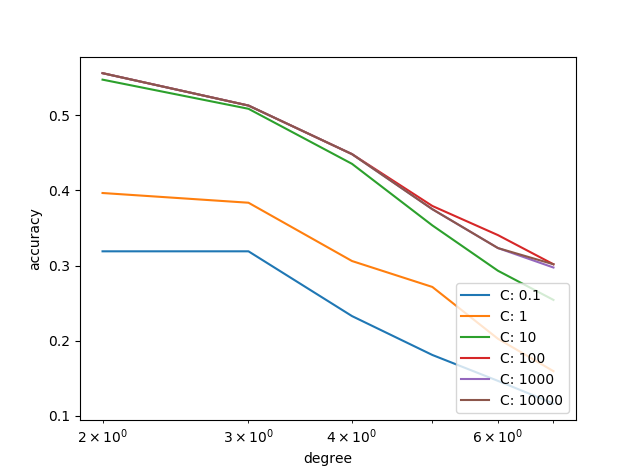
\includegraphics[scale=0.75]{img/svm/better_graphs/CFD_40i_poly.png}
\caption{Training score with varying polynomial degree and C parameter for 40 individuals}
\end{figure} 

The best score was obtained with degree = 2 and $C = 10^4$. With these parameters recognition rate reached ~52\%, which is still worse than SVM trained with Gaussian kernel.

\section{Tests on pictures captured in uncontrolled environment}

To test the algorithm the Labeled Faces in Wild database was used. The quality of images is much worse then in the previous examples, so the tests result are expected to be worse. 

Test was performed on 20 individuals with 30 pictures each. The training set for each person consists of 27 samples, 3 pictures were used to test the model. 

The results are presented below.

\begin{figure}[H]
\centering
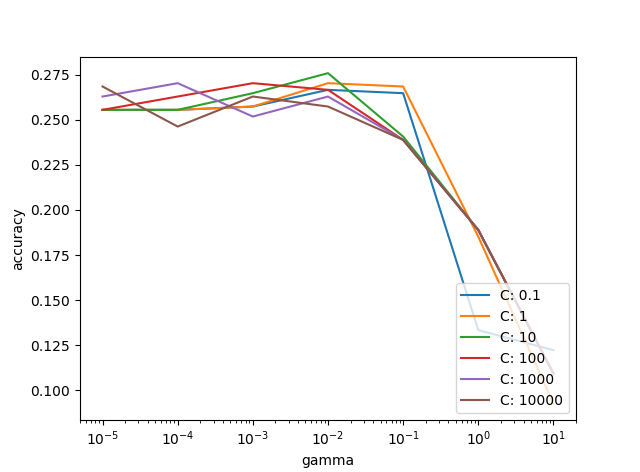
\includegraphics[scale=0.75]{img/svm/better_graphs/lwf_rbf.png}
\caption{Training score with varying gamma and C parameter for 20 individuals}
\end{figure} 

The best training score ($~0.278$) was obtained with with $C = 10$ and $\gamma = 0.01$
In this configuration SVM algorithm reached 26,6\% of recognition rate on the testing samples.


The same experiment was performed with usage of polynomial kernel. 
The influence of polynomial degree was examined and is presented on figure (???).

\begin{figure}[H]
\centering
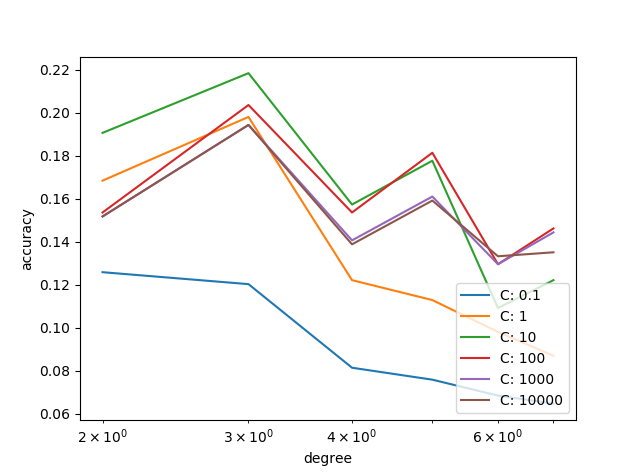
\includegraphics[scale=0.75]{img/svm/better_graphs/lwf_poly.png}
\caption{Training score with varying polynomial degree and C parameter for 20 individuals}
\end{figure} 

In this case, SVM obtained best results with third polynomial degree and $C = 10$. The obtained recognition rate was ~20\%.


\section{SVM summary}

To compare obtained results a tabular summary of the recognition rate for SVM algorithm with different kernels on each database is presented (Table 7.1).

\begin{table}[H]
	\centering
	\caption{A tabular summary of the recognition rate for SVM algorithm with different kernels on each database}
    \begin{tabular}{ | l | l | l | l |}
    \hline
    \rowcolor{lightgray}
    Database &  Gaussian kernel & Polynomial kernel\\ \hline
    CFD 20&  80\%  & 70\%\\ \hline
	CFD 40& $60\%$ & $52\%$ \\ \hline
    LFW & $26.6\%$ & $20\%$ \\ \hline
    \end{tabular}
\end{table}

From these tests we can conclude that the gaussian kernel allows us to obtain better results for every database. As expected, the results are significantly better for pictures captured in controlled environment and small amount of data. Even though SVM has an advantage of small computing time, the results do not meet the expectations of good facial recognition system. 

